\chapter{Giới thiệu và Tổng quan nghiên cứu}
\label{chap:introduction}

\section{Bối cảnh nghiên cứu: Đồ thị tri thức tiến hóa và mô hình nhúng}
\label{sec:background}

Trong kỷ nguyên bùng nổ thông tin và trí tuệ nhân tạo, Đồ thị tri thức (Knowledge Graph - KG) đã khẳng định vị thế là hạ tầng biểu diễn tri thức cốt lõi cho hàng loạt hệ thống thông minh, từ công cụ tìm kiếm ngữ nghĩa, hệ khuyến nghị cho đến các kiến trúc suy luận đa bước (Multi-Hop Reasoning) và mô hình ngôn ngữ lớn (Retrieval-Augmented Generation - RAG)~\cite{ji2021survey,nickel2016review}. Một đồ thị tri thức chuẩn tắc được mô hình hóa dưới dạng tập hợp các bộ ba quan hệ $\mathcal{G} = \{(h, r, t) \subseteq \mathcal{E} \times \mathcal{R} \times \mathcal{E}\}$, trong đó $\mathcal{E}$ đại diện cho tập thực thể (entities), $\mathcal{R}$ đại diện cho tập quan hệ ngữ nghĩa (relations), biểu thị rằng quan hệ $r$ tồn tại giữa thực thể đầu $h$ (head) và thực thể cuối $t$ (tail).

Tuy nhiên, trong thực tiễn đời sống xã hội, chính trị, kinh tế và khoa học, tri thức không bao giờ là một thực thể tĩnh tại. Tri thức nhân loại luôn vận động và biến đổi không ngừng theo thời gian: các sự kiện mới liên tục phát sinh, các nhân sự lãnh đạo thay đổi nhiệm kỳ, các quy định pháp luật được ban hành mới, bổ sung hoặc bãi bỏ, và các quan hệ đối ngoại giữa các quốc gia hay tổ chức tài chính tái cấu trúc liên tục~\cite{snodgrass1986temporal,jensen1999bitemporal}. Khái niệm \textbf{Đồ thị tri thức tiến hóa (Evolving Knowledge Graph - EKG)} ra đời nhằm phản ánh bản chất động này, trong đó đồ thị không còn là một snapshot đơn lẻ mà là một chuỗi các trạng thái quan sát theo trục thời gian thực nghiệm:
\begin{equation}
    \mathcal{G}_1 \subset \mathcal{G}_2 \subset \dots \subset \mathcal{G}_T
\end{equation}
hoặc tổng quát hơn là sự biến thiên liên tục bao gồm cả phép bổ sung bộ ba tri thức mới ($\Delta^+$), cập nhật thuộc tính ($\Delta^*$), và thu hồi tri thức lỗi thời ($\Delta^-$).

Để thực hiện các tác vụ tính toán phức tạp như dự đoán liên kết (Link Prediction), căn chỉnh thực thể (Entity Alignment) hay trả lời câu hỏi phức tạp (Complex Question Answering), các mô hình Nhúng đồ thị tri thức (Knowledge Graph Embeddings - KGE) đóng vai trò then chốt~\cite{bordes2013translating,sun2019rotate,trouillon2016complex}. Các kiến trúc KGE điển hình như TransE~\cite{bordes2013translating}, RotatE~\cite{sun2019rotate}, hay DistMult chuyển đổi các thực thể rời rạc $e \in \mathcal{E}$ và quan hệ $r \in \mathcal{R}$ thành các vector hoặc ma trận liên tục trong không gian vector đa chiều thấp $\mathbb{R}^d$:
\begin{equation}
    \mathbf{e} \in \mathbb{R}^d, \quad \mathbf{r} \in \mathbb{R}^d
\end{equation}
sao cho các quy luật tô-pô và ngữ nghĩa của đồ thị được bảo toàn dưới một hàm tính điểm khoảng cách hoặc tương đồng hình học cụ thể (ví dụ trong TransE, điều kiện chuyển dịch hình học đòi hỏi $\mathbf{h} + \mathbf{r} \approx \mathbf{t}$).

Khi đồ thị tri thức tiến hóa sang trạng thái mới $\mathcal{G}_{t+1}$, phương pháp chuẩn tắc trong kỹ nghệ công nghệ thông tin là tiến hành \textbf{tái huấn luyện định kỳ (Retraining)} mô hình KGE trên dữ liệu mới nhằm cập nhật biểu diễn vector cho các thực thể và mối quan hệ mới xuất hiện. Quá trình tái huấn luyện này là điều kiện tiên quyết để hệ sinh thái ứng dụng downstream (chẳng hạn như hệ thống QA) có thể tiếp cận được tri thức cập nhật nhất.

\section{Thách thức cốt lõi: Sự đan xen giữa Trôi dạt thực chất và Nhiễu tái huấn luyện}
\label{sec:core_challenge}

Mặc dù việc tái huấn luyện KGE theo thời gian là một nhu cầu bức thiết, cộng đồng khoa học máy tính đang đối mặt với một vấn đề nền tảng chưa được giải quyết thấu đáo: \textbf{Hiện tượng trôi dạt biểu diễn vector (Representation Drift) và sự đan xen không thể phân tách ngây thơ giữa tín hiệu và nhiễu ngẫu nhiên}~\cite{hamilton2016diachronic,kutuzov2018diachronic}.

Cụ thể, khi một mô hình KGE được huấn luyện lại trên snapshot mới $\mathcal{G}_{t+1}$, không gian vector biểu diễn tại thời điểm $t+1$ (ký hiệu là $\mathbf{E}^{(t+1)}$) sẽ không còn đồng nhất về hệ tọa độ hình học với không gian vector tại thời điểm $t$ (ký hiệu là $\mathbf{E}^{(t)}$). Sự sai khác vị trí vector của một thực thể $e$ giữa hai thời điểm, đo bằng khoảng cách hình học (như khoảng cách Cosine hoặc Euclid), bị chi phối bởi hai thành phần cơ bản:

\begin{figure}[htbp]
    \centering
    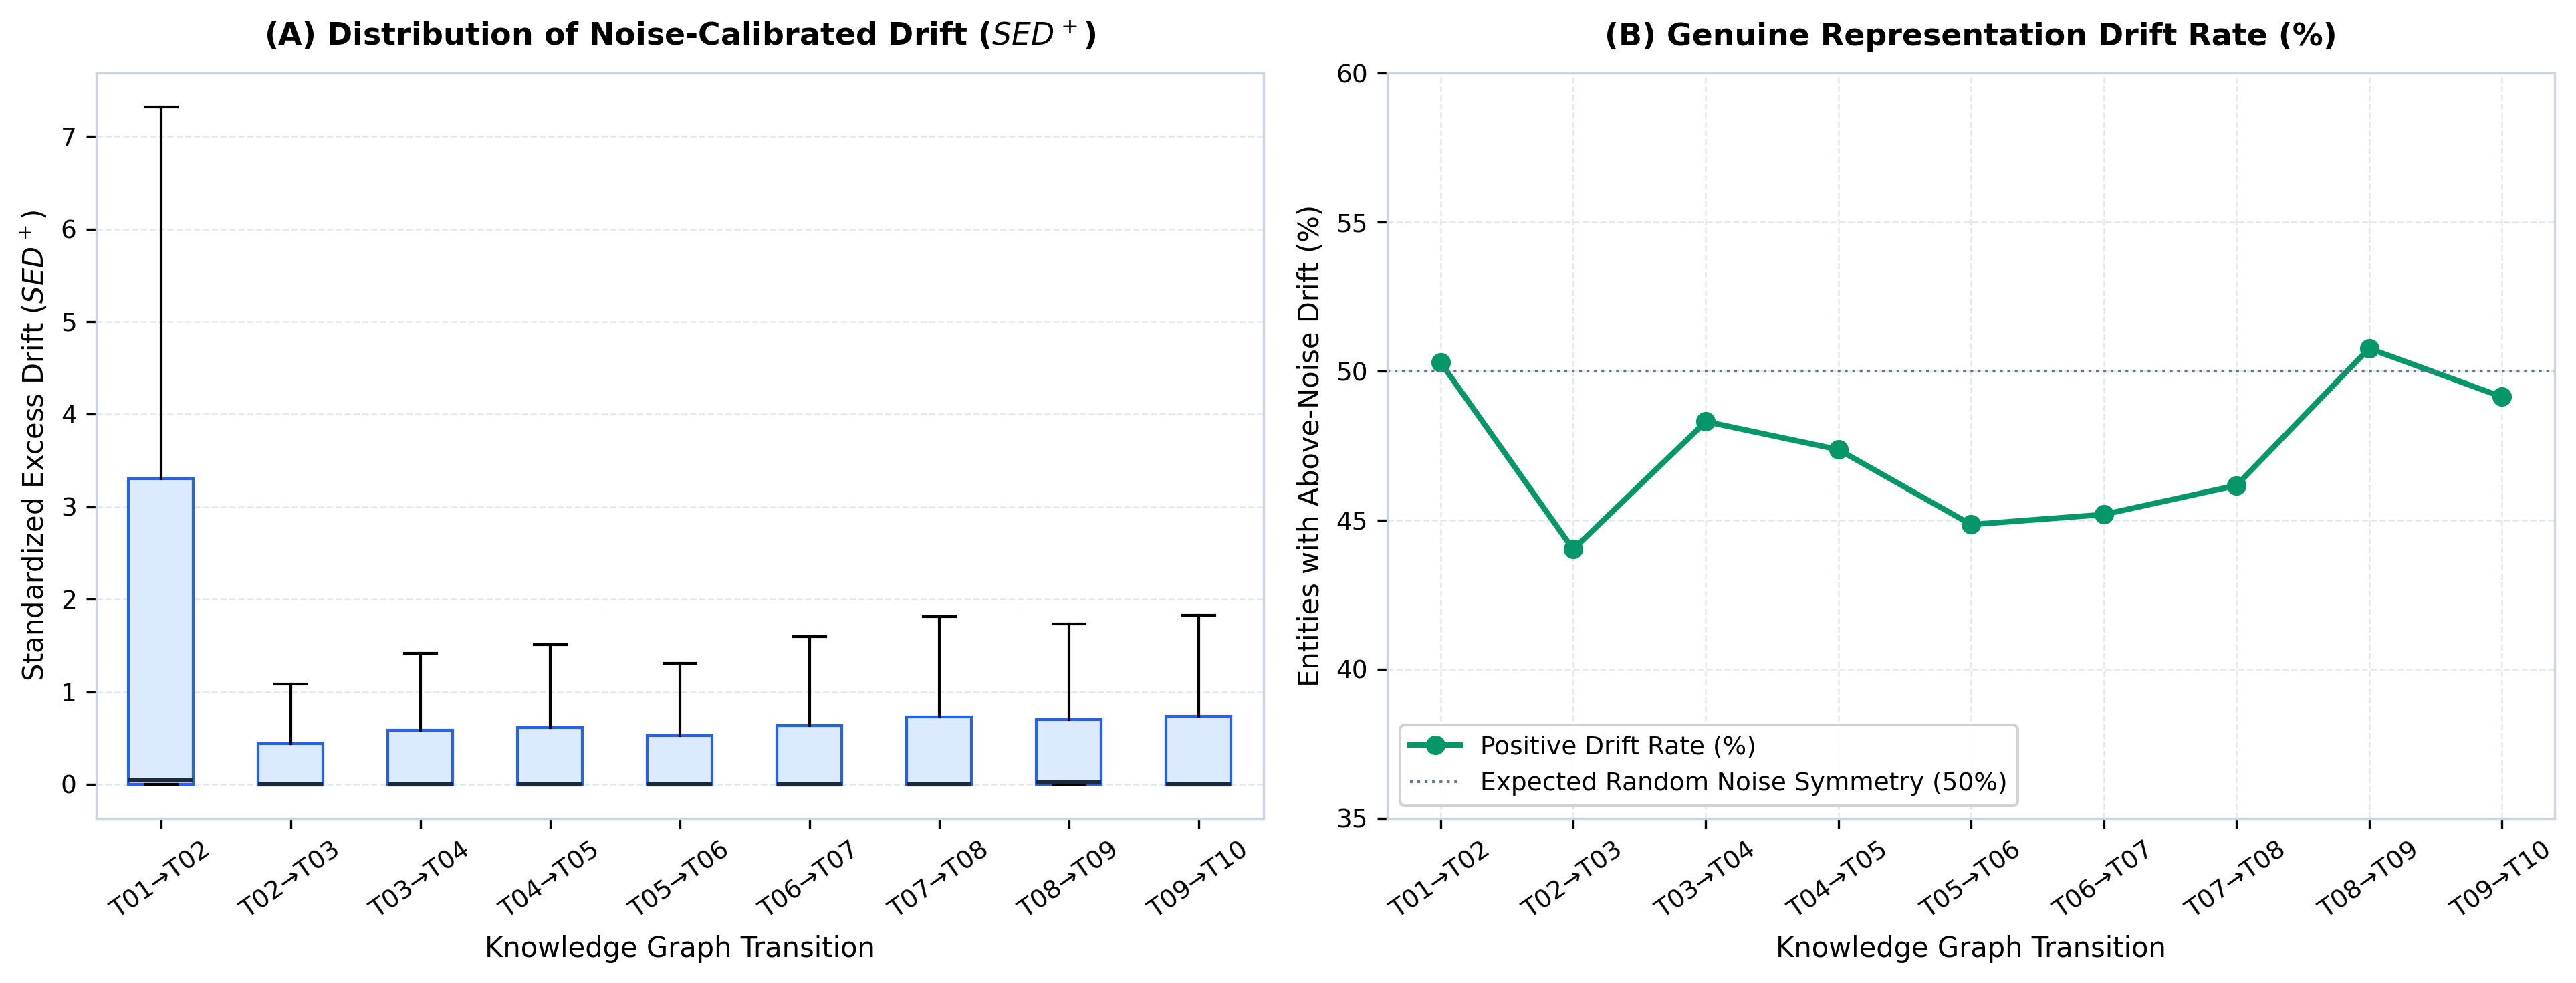
\includegraphics[width=0.92\textwidth]{figures/fig1_m2_representation_drift_sed_plus.png}
    \caption{Phân phối độ trôi biểu diễn có hiệu chỉnh nhiễu ($SED^+$) qua 9 bước chuyển đổi thời gian của đồ thị tri thức: (A) Biểu đồ hộp phản ánh độ trôi phân tán quanh 0; (B) Tỷ lệ thực thể có độ trôi vượt ngưỡng nhiễu nền dao động từ $42{,}1\%$ đến $53{,}6\%$.}
    \label{fig:intro_drift_distribution}
\end{figure}

\begin{enumerate}
    \item \textbf{Trôi dạt biểu diễn thực chất (Genuine Representation Drift):} Đây là sự dịch chuyển tọa độ thực tế bắt nguồn từ sự biến đổi tô-pô của đồ thị tri thức. Một thực thể tiếp nhận các cạnh mới, thay đổi vị trí trung tâm trong mạng lưới, hoặc quan hệ ngữ nghĩa của nó với các thực thể xung quanh bị tái cấu trúc. Đây chính là tín hiệu khoa học phản ánh sự tiến hóa của tri thức trong thế giới thực mà hệ thống cần nhận diện và khai thác.
    \item \textbf{Nhiễu ngẫu nhiên do tái huấn luyện (Retraining Stochastic Noise):} Kể cả khi cấu trúc đồ thị hoàn toàn không thay đổi ($\mathcal{G}_{t+1} \equiv \mathcal{G}_t$), nếu ta huấn luyện lại mô hình KGE bằng một hạt giống ngẫu nhiên (random seed) khác hoặc tráo đổi thứ tự mini-batch ngẫu nhiên, không gian vector nhúng thu được vẫn sẽ dịch chuyển mạnh mẽ. Nguyên nhân cốt lõi là do:
    \begin{itemize}
        \item Khởi tạo trọng số ngẫu nhiên ban đầu trong không gian đa chiều $\mathbb{R}^d$.
        \item Quá trình tối ưu hóa phi lồi (non-convex optimization) bằng Stochastic Gradient Descent (SGD) hoặc Adam hội tụ về các điểm cực tiểu cục bộ (local minima) hoàn toàn khác nhau.
        \item Tính bất biến quay và phản xạ (Rotational and Reflectional Invariance) của các hàm mất mát trong không gian Euclid (ví dụ: xoay toàn bộ không gian vector bằng một ma trận trực giao bất kỳ không làm thay đổi giá trị khoảng cách Euclid hay thứ hạng dự đoán nội bộ).
    \end{itemize}
\end{enumerate}

\paragraph{Hệ quả nghiêm trọng:}
Nếu một hệ thống phân tích dữ liệu trực tiếp đo khoảng cách vector thô giữa hai thời điểm $\delta(e) = \|\mathbf{e}^{(t+1)} - \mathbf{e}^{(t)}\|$ mà không thực hiện căn chỉnh không gian và hiệu chỉnh nhiễu ngẫu nhiên, hệ thống sẽ rơi vào tình trạng \textbf{ngộ nhận sai lầm (False Alarm)}: phần lớn độ dịch chuyển đo được thực chất chỉ là nhiễu ngẫu nhiên của bộ tối ưu hóa, chứ không phản ánh bất kỳ sự thay đổi tri thức nào. Điều này dẫn đến các suy luận sai lệch nghiêm trọng về chất lượng mô hình, gây bất ổn định cho hệ thống suy luận đa bước, và khiến các quyết định downstream trở nên không đáng tin cậy.

\section{Ba câu hỏi nghiên cứu cốt lõi (Research Questions)}
\label{sec:research_questions}

Xuất phát từ thách thức thực tiễn và lý thuyết nêu trên, đề tài tập trung giải quyết ba câu hỏi nghiên cứu tường minh (Core Research Questions):

\begin{quote}
    \textbf{Câu hỏi nghiên cứu 1 (RQ1 - Tách biệt tín hiệu khỏi nhiễu):} \\
    \textit{Liệu có thể xây dựng một khung đo lường hình học có khả năng chuẩn hóa và tách biệt một cách nhất quán độ trôi biểu diễn thực chất (Genuine Representation Drift) ra khỏi nhiễu ngẫu nhiên của quá trình tái huấn luyện KGE (Retraining Stochastic Noise) mà không vi phạm tính toàn vẹn thời gian hay không?}
\end{quote}

\begin{quote}
    \textbf{Câu hỏi nghiên cứu 2 (RQ2 - Tác động thống kê lên suy luận đa bước):} \\
    \textit{Sau khi đã hiệu chuẩn nhiễu nền và kiểm soát triệt để các biến cố định (Fixed Effects) cùng hiện tượng xáo trộn thực thể ngoài từ điển (OOV churn), độ trôi biểu diễn có mối quan hệ nhân quả hoặc tương quan thống kê có ý nghĩa với độ chính xác của các truy vấn suy luận đa bước (MRR/RR) hay không?}
\end{quote}

\begin{quote}
    \textbf{Câu hỏi nghiên cứu 3 (RQ3 - Cơ chế nâng cao năng lực của mô hình cập nhật):} \\
    \textit{Sự vượt trội về mặt hiệu năng của mô hình KGE được tái huấn luyện trong môi trường thế giới mở (Open-World) thực chất bắt nguồn từ việc tinh chỉnh tọa độ biểu diễn vector của các thực thể đã biết, hay chủ yếu xuất phát từ việc mở rộng độ bao phủ thực thể (Entity Coverage Expansion) giúp triệt tiêu hình phạt OOV?}
\end{quote}

\section{Mục tiêu và các đóng góp kỳ vọng của đề tài}
\label{sec:contributions}

Đề tài đặt mục tiêu nghiên cứu và đạt được ba đóng góp khoa học chính (Contributions):

\begin{enumerate}
    \item[\textbf{C1.}] \textbf{Khung đo lường hình học hiệu chuẩn nhiễu (Noise-Calibrated Geometric Drift Framework):}
    Xây dựng thuật toán căn chỉnh không gian tối ưu Centered Orthogonal Procrustes SVD trên tập mỏ neo bền vững (persistent anchors), kết hợp mô hình hóa phân phối giả thuyết không thực nghiệm (Same-Snapshot Empirical Null) thông qua việc huấn luyện mô hình đa seed cố định (13, 37, 101) và kỹ thuật loại trừ mục tiêu Leave-Target-Out (LTO). Đóng góp này mang lại chỉ số $SED^+$ (Standardized Excess Drift), cho phép định lượng chính xác phần trôi dạt vượt trên phương sai nhiễu ngẫu nhiên.

    \item[\textbf{C2.}] \textbf{Thiết kế thực nghiệm kinh tế lượng bảng lặp lại (Recurring Longitudinal QA Panel):}
    Thiết lập bộ dữ liệu đánh giá suy luận đa bước gồm 147 câu hỏi phức tạp theo dõi cố định qua 10 snapshot (9 bước chuyển đổi thời gian, tổng cộng 1.323 quan sát). Áp dụng mô hình hồi quy Two-Way Fixed Effects (TWFE) kết hợp suy diễn thống kê bằng Wild Cluster Bootstrap (WCB) với cụm bước chuyển đổi thời gian, nhằm kiểm định giả thuyết $H_1$ về tác động của độ trôi biểu diễn lên chất lượng suy luận mà không bị ảnh hưởng bởi các yếu tố gây nhiễu bất biến theo thời gian hoặc theo câu hỏi.

    \item[\textbf{C3.}] \textbf{Phân tích phân rã thiên lệch OOV và kiểm định ngụy tạo (Falsification Testing):}
    Thực hiện kiểm định ngụy tạo thông qua biến trôi dạt giả cùng thời điểm ($D^{pseudo}$), chứng minh phương pháp đo lường không sinh ra hiệu ứng giả mạo dưới tác động của nhiễu tái huấn luyện thuần túy. Đồng thời, giải mã cơ chế tác động thông qua phân tích đối chiếu giữa không gian kín (Seen-at-T1) và không gian mở (Open-World), phân rã định lượng khoảng cách thiên lệch OOV (OOV Churn Penalty Gap).
\end{enumerate}

\section{Phạm vi nghiên cứu MVR (Minimum Defensible Research)}
\label{sec:mvr_scope}

Để đảm bảo tính khả thi, tính chặt chẽ học thuật và khả năng bảo vệ thành công của một công trình nghiên cứu khoa học cấp trường/cấp bộ môn, đề tài tuân thủ nghiêm ngặt nguyên tắc \textbf{Phạm vi nghiên cứu tối thiểu có thể bảo vệ (Minimum Defensible Research - MVR)}:

\begin{itemize}
    \item \textbf{Mô hình KGE cơ sở:} Sử dụng kiến trúc TransE chuẩn tắc với khoảng cách $L_2$ (TransE-L2) trong không gian $d=64$ chiều, được huấn luyện tối ưu hóa có kiểm soát bằng thuật toán Adam qua 50 epochs, learning rate $0{,}01$, margin $\gamma = 1{,}0$. Đề tài không sáng tạo thêm kiến trúc KGE mới mà tập trung toàn bộ vào độ tin cậy của phép đo lường trôi dạt.
    \item \textbf{Các hạt giống ngẫu nhiên cố định:} Khóa cứng ba seed tiêu chuẩn đại diện cho tính ngẫu nhiên của quá trình huấn luyện: $\{13, 37, 101\}$. Mọi phép ước lượng nhiễu nền đều được tính toán trên 6 cặp cross-seed có đối chứng tại cùng một snapshot.
    \item \textbf{Chuỗi 10 Snapshot thời gian:} Chuỗi tiến hóa gồm 10 snapshot $T_{01}, T_{02}, \dots, T_{10}$ trích xuất từ dữ liệu thời gian thực (báo chí chính thống, xác thực chứng cứ không rò rỉ tương lai - No Future Evidence). Quy mô tăng trưởng từ 121 quan hệ (167 thực thể) tại $T_{01}$ lên 1.205 quan hệ (1.389 thực thể) tại $T_{10}$.
    \item \textbf{Các bất biến khoa học cốt lõi (Hard Scientific Invariants):}
    \begin{itemize}
        \item \textit{INV-01 (Không rò rỉ tương lai):} Không có bất kỳ sự kiện nào xảy ra sau mốc cutoff của snapshot được phép đưa vào dữ liệu huấn luyện.
        \item \textit{INV-02 (Tách biệt trục thời gian):} Phân biệt tuyệt đối giữa thời gian thế giới thực (`valid\_from`, `valid\_to`), thời gian quan sát chứng cứ (`evidence\_observed\_at`), và thời gian thu thập dữ liệu kỹ thuật (`ingested\_at\_real`).
        \item \textit{INV-04 (Tái lập tất định):} Mọi kết quả từ tiền xử lý, huấn luyện đến phân tích kinh tế lượng đều có khả năng tái lập bit-to-bit (exact SHA-256 match).
    \end{itemize}
\end{itemize}

Bố cục các chương còn lại của báo cáo được tổ chức như sau: Chương~\ref{chap:theoretical_foundations} trình bày cơ sở lý thuyết toán học và kinh tế lượng; Chương~\ref{chap:system_architecture} mô tả kiến trúc hệ thống và quy trình thực nghiệm khép kín; Chương~\ref{chap:empirical_results} công bố toàn bộ kết quả thực nghiệm định lượng; Chương~\ref{chap:discussion} thảo luận chuyên sâu về ý nghĩa học thuật và bảo vệ kết quả; và Chương~\ref{chap:conclusion} đúc kết đóng góp, nêu rõ hạn chế và mở ra hướng nghiên cứu tiếp theo.
